\section{Conclusions}
\label{sec:conclusions}

%Neutral current (NC) and charged current (CC) neutrino-nucleus coherent pion production are important backgrounds to neutrino oscillation measurements.  Current and future long baseline oscillation experiments, which aim to determine the neutrino mass hierarchy and measure the difference between neutrino and antineutrino oscillations, operate at neutrino energies in the range 1.0 $\lesssim$ \enu $\lesssim$ 10 GeV.  Measurements of coherent pion production at these energies are needed to constrain models of coherent pion production used by oscillation experiments.

%Ideally, coherent interactions are isolated using only model independent features of coherent scattering, which are the production of a lepton and pion in the forward direction and the nucleus remaining in its initial state.  The squared four-momentum transferred to the nucleus, \tabs, is necessarily small for the nucleus to remain intact and is a strong indicator of coherent scattering.  \tabs cannot be measured for NC coherent scattering since the final state lepton is not observed.  Since \tabs is not available, NC coherent pion production measurements make assumptions about the pion kinematics in isolating NC coherent interactions and have large uncertainties as a result.  With a capable detector, the kinematics of CC coherent interactions, including \tabs, can be measured completely.  This enables measurements of CC coherent pion production to be made without assumptions of the coherent scattering kinematics, which then allows tests of the kinematic predictions of coherent models.  This situation increases the importance of CC coherent pion production measurements which, in the PCAC picture of coherent scattering, provide a constraint on the NC reaction.

%Neutrino oscillation experiments use the coherent pion production model by Rein and Sehgal.  The predictions of the Rein-Sehgal model are in good agreement with early measurements of \numu and \numubar CC coherent pion production, the majority of which were made a $\enu\gtrsim$ 10 GeV.  Recently, the K2K and SciBooNE experiments found no evidence for \numu CC coherent pion production at $\enu\lesssim$ 2 GeV, and reported upper limits on the cross section that are lower than the Rein-Sehgal model prediction.  Neither K2K nor SciBooNE were able to measure \tabs.  The non-observation of CC coherent pion production $\enu\lesssim$ 2 GeV forced the T2K experiment, which operates at $\enu\sim$ 1 GeV, to apply a 100\% uncertainty on the predicted CC coherent pion production rate in their oscillation measurements.

This paper has reported measurements of \numu and \numubar CC coherent pion production on carbon from \minerva data.
The cross sections were measured for neutrino energies in the range 2.0 $<$ \enu $<$ 20 GeV, where
$\langle\enu\rangle\approx$ 4 GeV.  The measurements were made by isolating coherent interactions using the model
independent experimental signature of CC coherent scattering, which consists of a charged lepton and pion in the
forward direction, no evidence of nuclear breakup, and small \tabs.
A data-driven constraint on the background prediction was designed to minimize dependence on modeling nuclear
effects which are poorly understood.  Unambiguous signals of \numu and \numubar CC coherent pion production above
the predicted background were observed at small \tabs.  The cross sections \sigenu, \dsigdqsq, \dsigdepi
and \dsigdthetapi were measured for both \numu and \numubar CC coherent pion production.  \enu, \qsq, \epi, \thetapi
and \tabs characterize the kinematics of coherent scattering completely.

The measured cross sections were compared to the Rein-Sehgal and Berger-Sehgal coherent models, which are both
based on Adler's PCAC theorem.  The Rein-Sehgal model calculates the pion-nucleus elastic scattering cross section
from pion-nucleon scattering data.  The Berger-Sehgal model calculates the pion-nucleus scattering cross section
from pion-carbon elastic scattering data and scales the cross section to other nuclei.  Both the Rein-Sehgal and
Berger Sehgal predictions agree with the measured total cross-section as a function of neutrino energy in the \numu and \numubar samples.  For both
\numu and \numubar, the measured \dsigdepi (\dsigdthetapi) exhibits a harder (more forward) spectrum than the
Rein-Sehgal and Berger-Sehgal predictions, which suggests that both models miscalculate the pion-nucleus elastic
scattering cross section.  The Rein-Sehgal predictions were brought into better agreement with the measured
\dsigdepi and \dsigdthetapi by weighting the predicted rate of interactions with $\epi<$ 500 MeV by 50\%.  For
both \numu and \numubar, the Rein-Sehgal and Berger-Sehgal predictions are similar in shape to the measured \dsigdqsq,
which supports the axial vector dipole parameterization of the \qsq dependence of the coherent cross section.

PCAC coherent models assume coherent scattering is a purely axial vector process.  PCAC coherent models therefore
predict equal cross sections for neutrinos and antineutrinos.  To test this prediction, the measured \numu and
\numubar cross sections were compared, where the \numu differential cross sections were weighted to the \numubar flux.
No significant differences between the \numu and \numubar cross sections were observed.

Since the \minerva scintillator contains equal numbers of carbon and hydrogen atoms, diffractive pion production on
hydrogen is a possible contribution to the measured cross sections.  Diffractive pion production is indistinguishable
from coherent pion production when the recoil proton is undetected.  A search for diffractive pion production within
the coherent pion production candidate samples was performed by looking for ionization from a recoil proton near the
interaction vertex.  Neither the \numu nor \numubar coherent candidate samples exhibited evidence for such a diffractive
contribution.
%The absence of diffractive pion production in the coherent pion candidate samples is understood from the diffractive acceptance of the vertex energy cut and the \tabs dependence of the diffractive cross section.

\begin{figure}[tpb]
\centering
%\includegraphics[width=0.9\columnwidth]{figures/CrossSection/h_Ev_Final_XSec_WorldData_ThetaPiCor_FluxConstrained_WeightedSignalModel_neutrino.pdf}
%\includegraphics[width=0.9\columnwidth]{figures/CrossSection/h_Ev_Final_XSec_WorldData_ThetaPiCor_FluxConstrained_WeightedSignalModel_antineutrino.pdf}
%\caption[Compilation of measurements of CC coherent pion production including this result]{Compilation of measurements of the \numu (top) and \numubar (bottom) CC
%	coherent pion production cross sections as a function of energy.  All results are scaled to A=12 (carbon) assuming $\sigma\propto A^{1/3}$. }
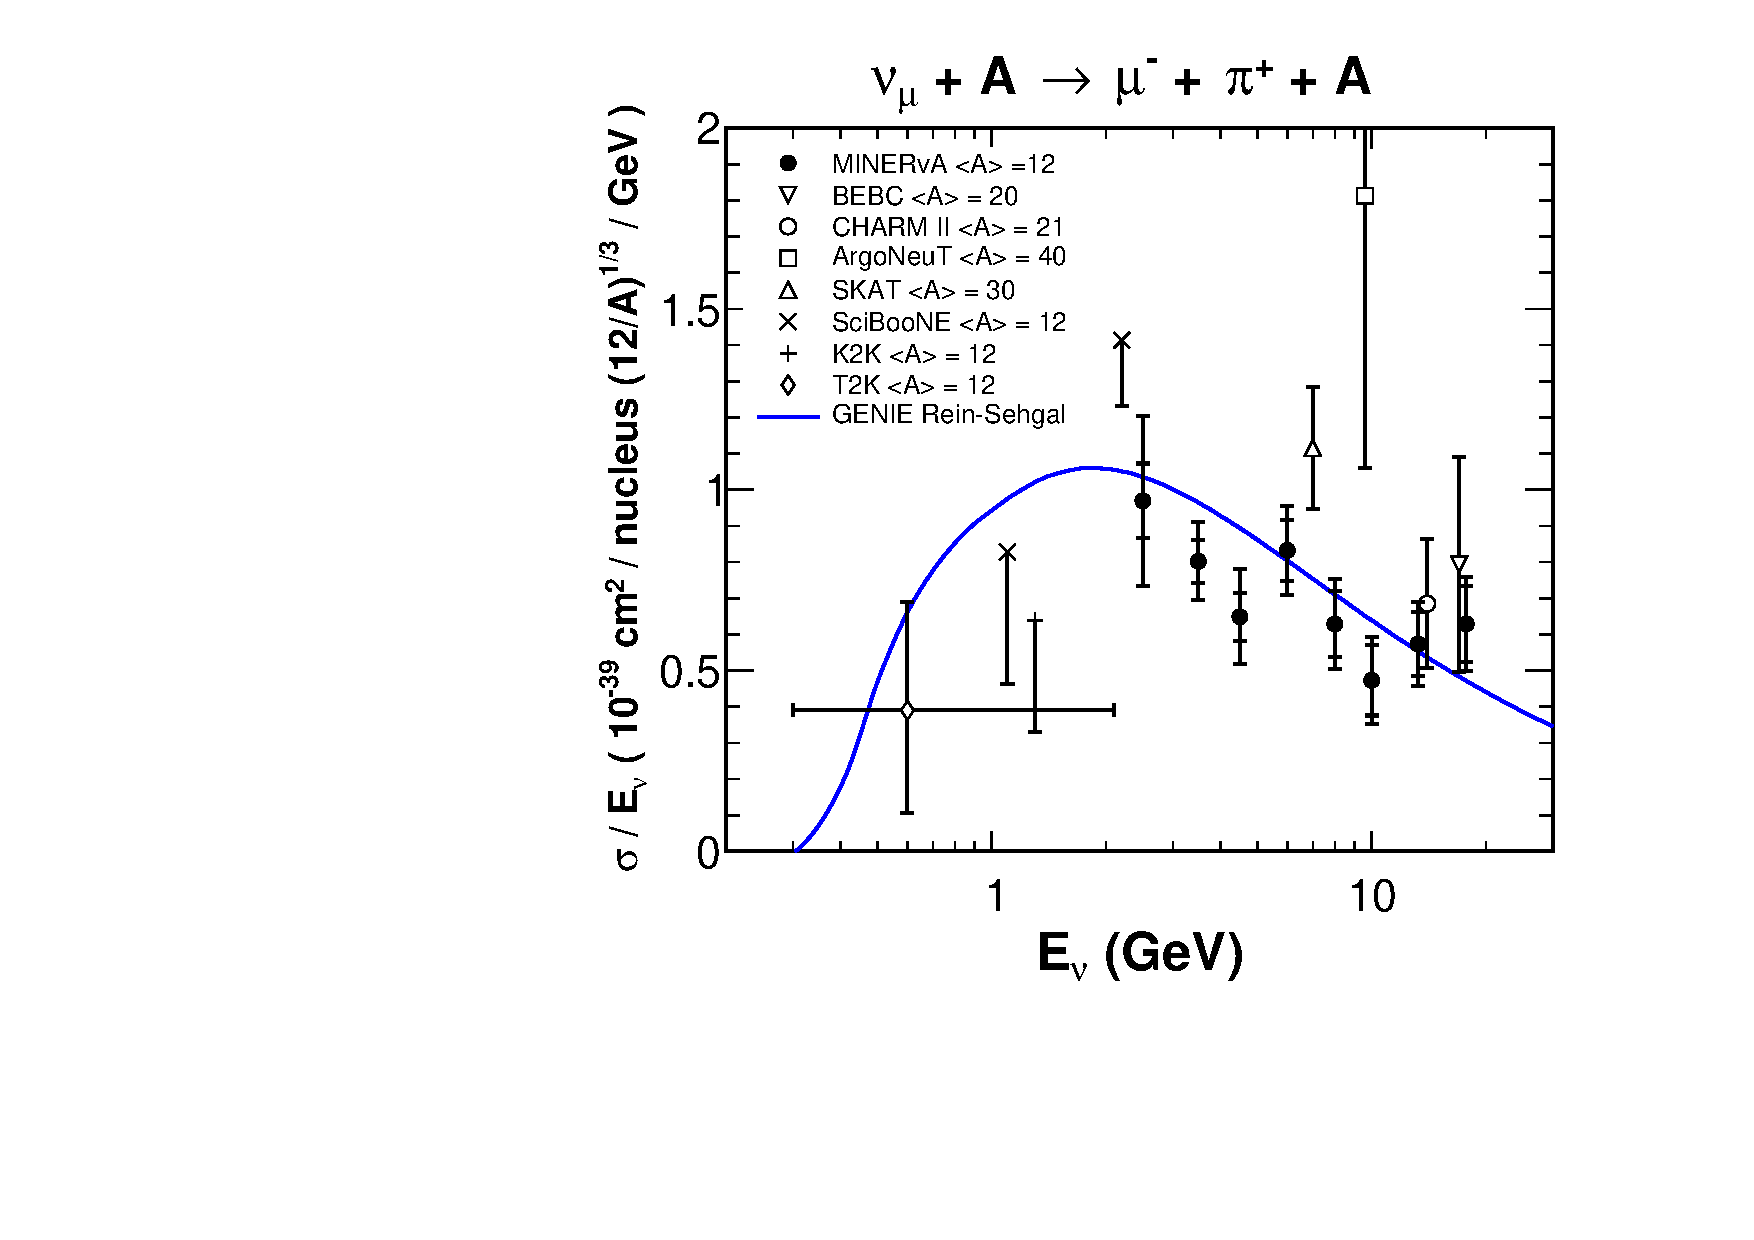
\includegraphics[width=0.9\columnwidth]{figures/CrossSection/h_Ev_Final_XSec_WorldData_ThetaPiCor_FluxConstrained_WeightedSignalModel_neutrino_sigmaOverE.pdf}
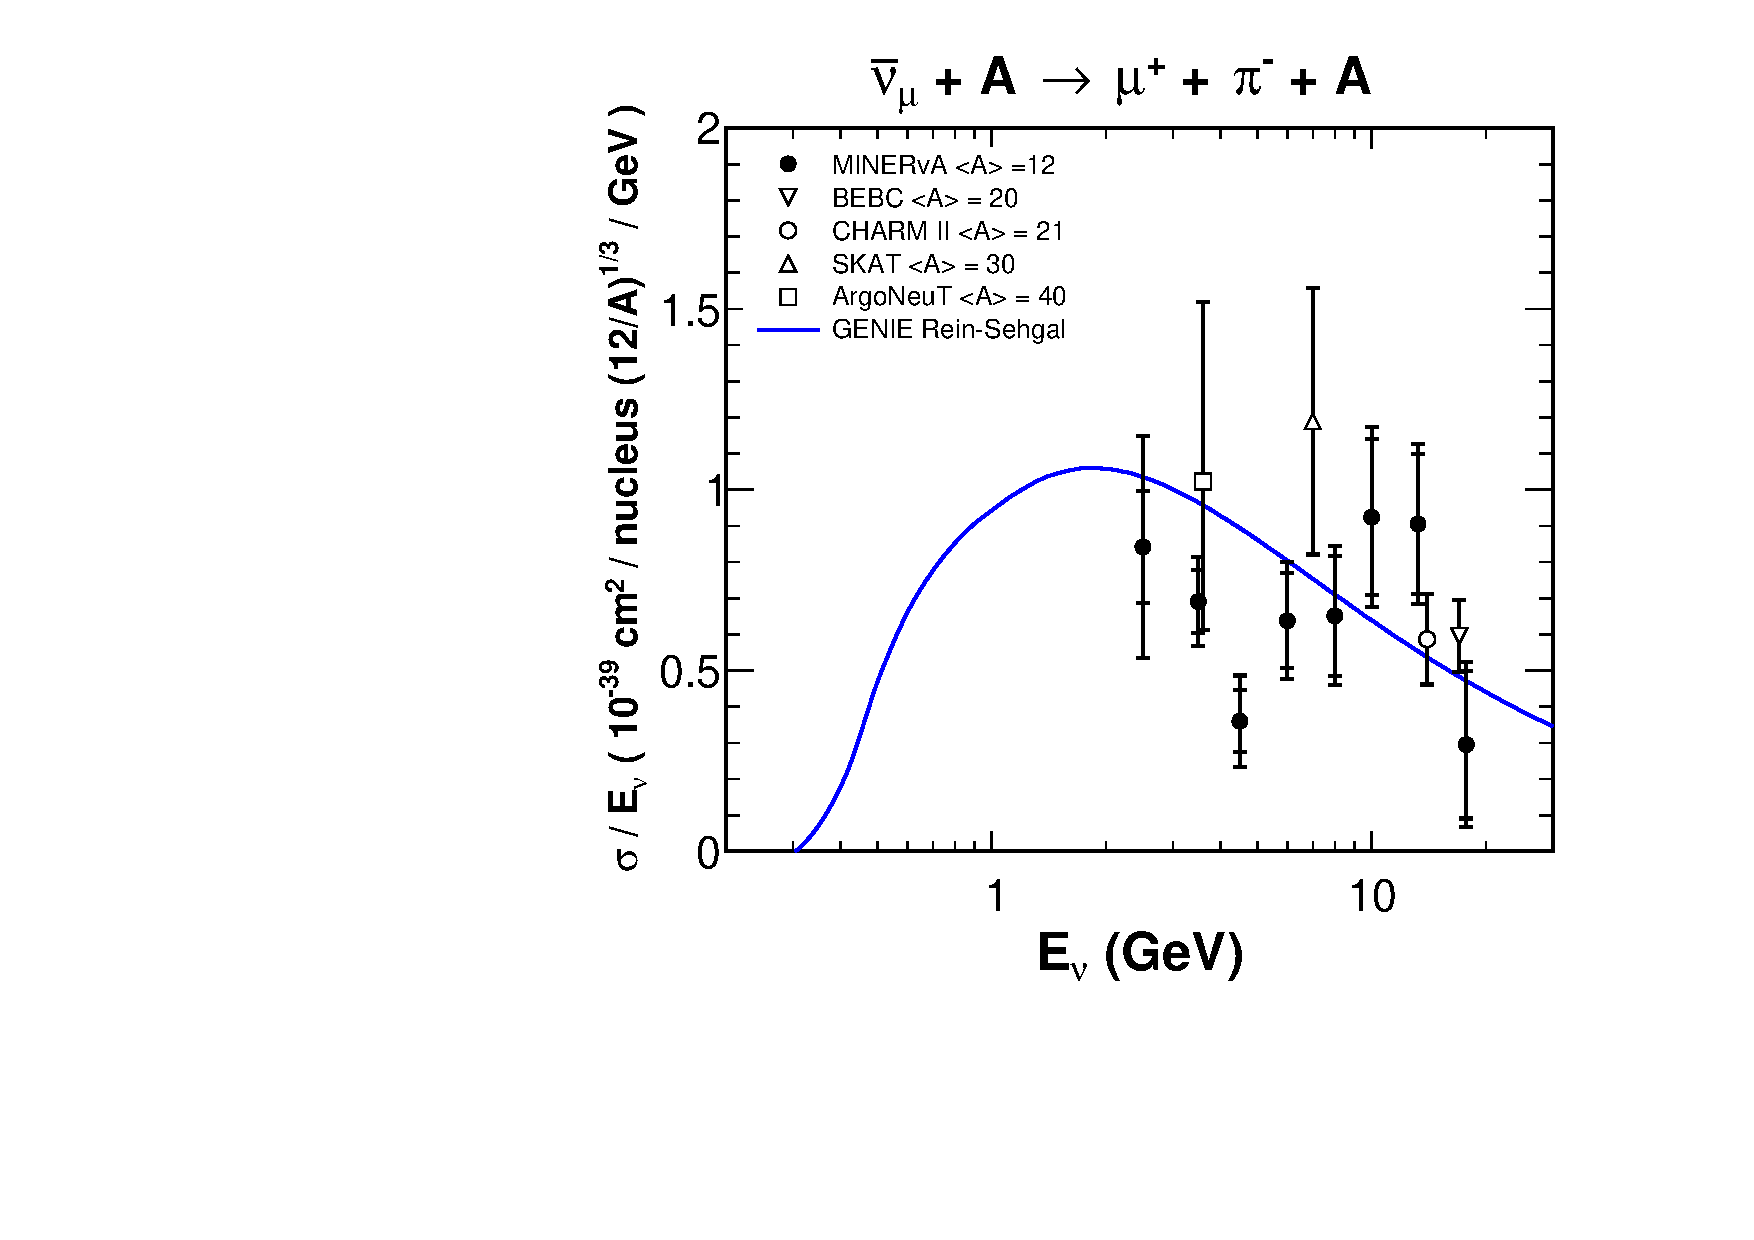
\includegraphics[width=0.9\columnwidth]{figures/CrossSection/h_Ev_Final_XSec_WorldData_ThetaPiCor_FluxConstrained_WeightedSignalModel_antineutrino_sigmaOverE.pdf}
\caption[Compilation of measurements of CC coherent pion production including this result]{Compilation of measurements of the \numu (top) and \numubar (bottom) CC
	coherent pion production cross sections as a function of energy.  Cross sections divided by neutrino energy is shown for display convenience.  All results are scaled to A=12 (carbon) assuming $\sigma\propto A^{1/3}$. }
\label{fig:coh_cc_compilation}
\end{figure}

The measurements reported in this paper are a significant addition to the world data set of neutrino-nucleus
coherent pion production.  Cross sections as a function of neutrino energy from the world data set are shown in Fig.~\ref{fig:coh_cc_compilation}.
This includes recent measurements from ArgoNEUT~\cite{bib:coh_cc_argo} and T2K~\cite{bib:coh_cc_t2k} which are significantly less precise than the
MINERvA measurements and do not report differential cross sections.  The T2K measurement, however, plays a special role here in that it shows
consistency of the cross section at lower energies than accessible by MINERvA with the $d\sigma/dE_\pi$ at low pion energies below the prediction
of the GENIE Rein-Sehgal model. 

The MINERvA measurements presented in this paper provide the most precise information about charged-current coherent pion production below neutrino
energies of 15 GeV.  The measurements provide constraints on not only the total rate, but also on the
kinematics of coherent pion production.  These measurements can be used to benchmark coherent pion production models
from production threshold up to neutrino energies of 20 GeV, which is the most important energy regime for current and future neutrino oscillation
experiments.
